\input{permve-ntnu-latex-assignment.tex}

\usepackage{float}

\title{	
\normalfont \normalsize 
\textsc{Norwegian University of Science and Technology\\IT3105 -- Artificial Intelligence Programming}
\horrule{0.5pt} \\[0.4cm]
\huge Module 2:\\Combining Constraint-Satisfaction Problem-Solving with Best-First
Search\\
\horrule{2pt} \\[0.5cm]
}

\author{Per Magnus Veierland\\permve@stud.ntnu.no}

\date{\normalsize\today}

\newacro{CSP}{Constraint Satisfaction Problem}
\newacro{GAC}{General Arc Consistency}

\begin{document}

\maketitle

\section*{Generality of A* implementation}

The \ac{CSP} and \ac{GAC} related code is implemented in the \texttt{vi.csp} namespace. A \texttt{Network} object holds all \texttt{Variable} and \texttt{Constraint} objects, as well as a \texttt{domains} mapping from \texttt{Variable} objects to the domains of the variables. The values within a domain can be of any type. Also within the \texttt{vi.csp} namespace are the functions implementing \textsc{REVISE*} and \ac{GAC}. None of this code is tied to search code; and it can be used in full isolation where needed.

A \texttt{Constraint} holds the list of variables it is linked to, as well as a condition which can be evaluated. A \texttt{Variable} has an identity which can be of any type suiting the problem, as well as the list of contraints it is involved in.

Fusing the \ac{GAC} algorithm with A* is done by the \texttt{vi.search.gac.Problem} class, which is constructed from a \texttt{vi.csp.Network} object -- see Figure~\ref{figure:vi_astar_gac}. The \texttt{Network} object serves as the state of each search node. The \texttt{Problem} class provides the methods \texttt{goal\_test}, \texttt{heuristic}, \texttt{initial\_node}, and \texttt{successors} -- which forms the interface to the A* search class.

No problem specific code exists in the \texttt{vi.search.gac.Problem} class. It has a goal test which checks that all domains in the current state has a size of one. It has a heuristic which returns the sum of the length of all domains minus one. The initial search node returned from the \texttt{Problem} class is simply the initial network passed through one iteration of the \texttt{general\_arc\_consistency} function.

The crucial part of the \texttt{Problem} class implementation lies in the \texttt{successors} method. All successors generated from a search node is based on assumptions made about a single variable. The implementation selects the variable which has the smallest domain which contains more than one value. A successor state is generated for each value in the assumed variable's domain. The \ac{GAC} domain filtering loop is then warm rebooted to revise the domains of all variables which share a constraint with the assumed variable.

\begin{figure}[H]
\centering
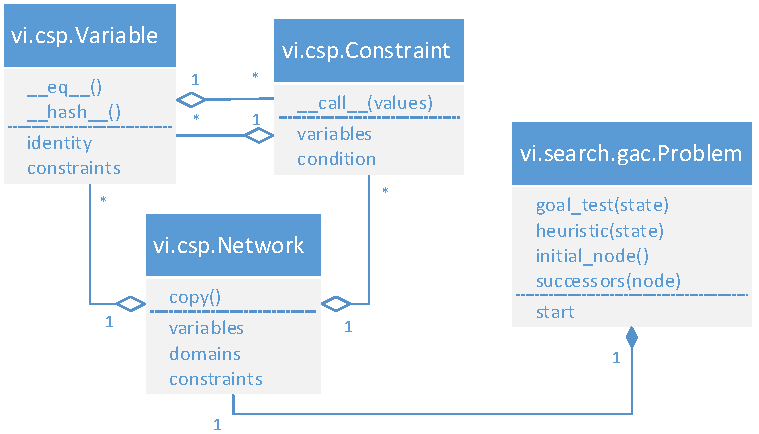
\includegraphics[scale=0.7]{images/vi_astar_gac}
\caption{VI CSP and A*-GAC classes}
\label{figure:vi_astar_gac}
\end{figure}

\section*{Generality of A*-GAC implementation}

The input to the vertex coloring problem is a pure graph description; with no direct relation to the vertex coloring problem. The file input is parsed and used to construct a graph using the \texttt{vi.graph.Vertex}, \texttt{vi.graph.Edge} and \texttt{vi.graph.Graph} classes; which are fully problem independent.

A single function in the \texttt{vi.app.vertex\_coloring} namespace takes the \texttt{vi.graph.Graph} object constructed from the file input, together with a $K$-value describing the number of colors -- and builds a \texttt{vi.csp.Network} which contains the variables, constraints and domains which describes the vertex coloring problem. It simply generates one \texttt{Variable} for each \texttt{Vertex} object; with the \texttt{Vertex} object as the variable's identity. For each \texttt{Edge} object a \texttt{Constraint} object is built which binds the two \texttt{Variable} objects associated with each \texttt{Vertex} in the edge together. The condition assigned to each constraint simply verifies that the values assigned to each of the two variables are different.

\section*{Constraint network}

A constraint network consists of constraints, variables, and domains. Much of this information is identical between search states. The assignment specifies that the variables and constraints will be the same in all states. The difference between the states is the sizes of the domains belonging to the different variables.

The constraint network is represented with the \texttt{vi.csp.Network} class. It holds a all variables involved in the network; a list of all constraints involved in the network; and it holds the mapping from variables to their respective domains. It is important to note that there is no direct connection from a \texttt{Variable} instance to its domain; this connection is only made by the mapping which exists in each \texttt{Network} instance. A \texttt{Network} instance is the state for each search node in the A*-GAC implementation. However importance is place on how the \texttt{Network} object is copied and which data is shared between states.

All \texttt{vi.csp.Network} instances which belong to the same problem share the list of variables and the list of constraints. There is only a single list of variables and a single list of constraints; and each instance of the \texttt{Network} class points to the same two lists. It is still important that each instance contains these two pointers since \texttt{Network} objects belonging to different problems will necessarily maintain different lists of variables and constraints.

The \texttt{Network.copy()} member function returns a new instance of the class which points to the same lists of variables and constraints; but which takes a shallow copy of the domains mapping. This means that no actual domains are copied, only the mapping from variables to domains. When applying the GAC algorithm to a \texttt{Network} instance, the relevant mappings of revised domains is updated to point at the new revised domain for the involved variables. This ensures high reuse in representation and avoids redundant information, without increasing the complexity of the implementation.

\section*{Code chunks}

In the given implementation a \texttt{Constraint} class instance holds a single condition and a list of variables involved in the condition. The condition must be callable and must accept one parameter. The parameter passed to a condition is a mapping of variables to specific values for all variables involved in the constraint. This makes the \texttt{Constraint} interface very general and allows any hashable type to be used as the \texttt{Variable} identity and in variable domains.

Since all variables involved in a \texttt{Constraint} is explicitly specified it is easy to generate the required permutations of values from variable domains in the \textsc{REVISE*} algorithm.

The interface was chosen for its semantical purity and generality. It can be used with both interpreters parsing user input as well as direct \texttt{eval} approaches simply by adding code to build the necessary \texttt{Constraint} objects and callable conditions. Since no parsing of user input was necessary for the given problem; only a simple lambda verifying the inequality of two variable values in the given value set was used.

\end{document}

